\documentclass{article}
\usepackage[T1]{fontenc}
\usepackage[polish]{babel}
\usepackage[utf8]{inputenc}
\usepackage[none]{hyphenat}
\usepackage{amsmath}
\usepackage{hyperref}
\usepackage{graphicx}
\usepackage{fancyhdr}
\usepackage{lastpage}

\pagestyle{fancy}
\fancyhf{}
\cfoot{\thepage\ / \pageref{LastPage}}

\graphicspath{ {images/p1/} }

\begin{document}

\begin{titlepage}
    
    \begin{center}
        \Large
            Politechnika Warszawska 
        
            Wydział Elektryczny 
        
            Kierunek Informatyka stosowana
        \vfill
        \Huge \textsc{Kamera Wirtualna}
        
        \Large 
            Sprawozdanie z pierwszej części projektu
        
            Grafika Komputerowa
    \end{center}
    \vfill



    \begin{center}
        \Large 
            Mateusz Ciupa
        
            291062
    \end{center}

    \begin{center}
        \Large	\today
    \end{center}

\end{titlepage}

\tableofcontents

\newpage

\section{Wstęp}

    Celem pierwszej części projektu było zaimplementowanie kamery wirtualnej w dowolnym 
    języku. Kamera powinna umożliwiać dokonywania translacji (lewo, prawo, góra i dół), 
    rotacji wokół trzech osi oraz operacji zoom. Ćwiczenie zostało wykonane przy użyciu 
    języka \textbf{JavaScript} oraz elementu \textbf{Canvas} języka HTML. Materiały 
    (w tym technika wykonania) zostały operte na książce: \textit{Fundamentals Of Computer
    Graphics - Peter, Shirley, Steve Marschner}.

\section{Opis obiektów}

    Obiekty, które są rysowane na ekranie, są bryłami, które składają się z krawędzi
    (dwóch punktów połączonych linią). Wszystkie punkty są określone przez
    współrzędne jednorodne trójwymiarowej przestrzeni (x, y, z, 1).

\section{Operacje kamery}

    Operacje są wykonywane poprzez przemnożenie wszystkich punktów tworzących obiekty
    z odpowiednimi macierzami (4x4).

    \begin{figure}[h]
        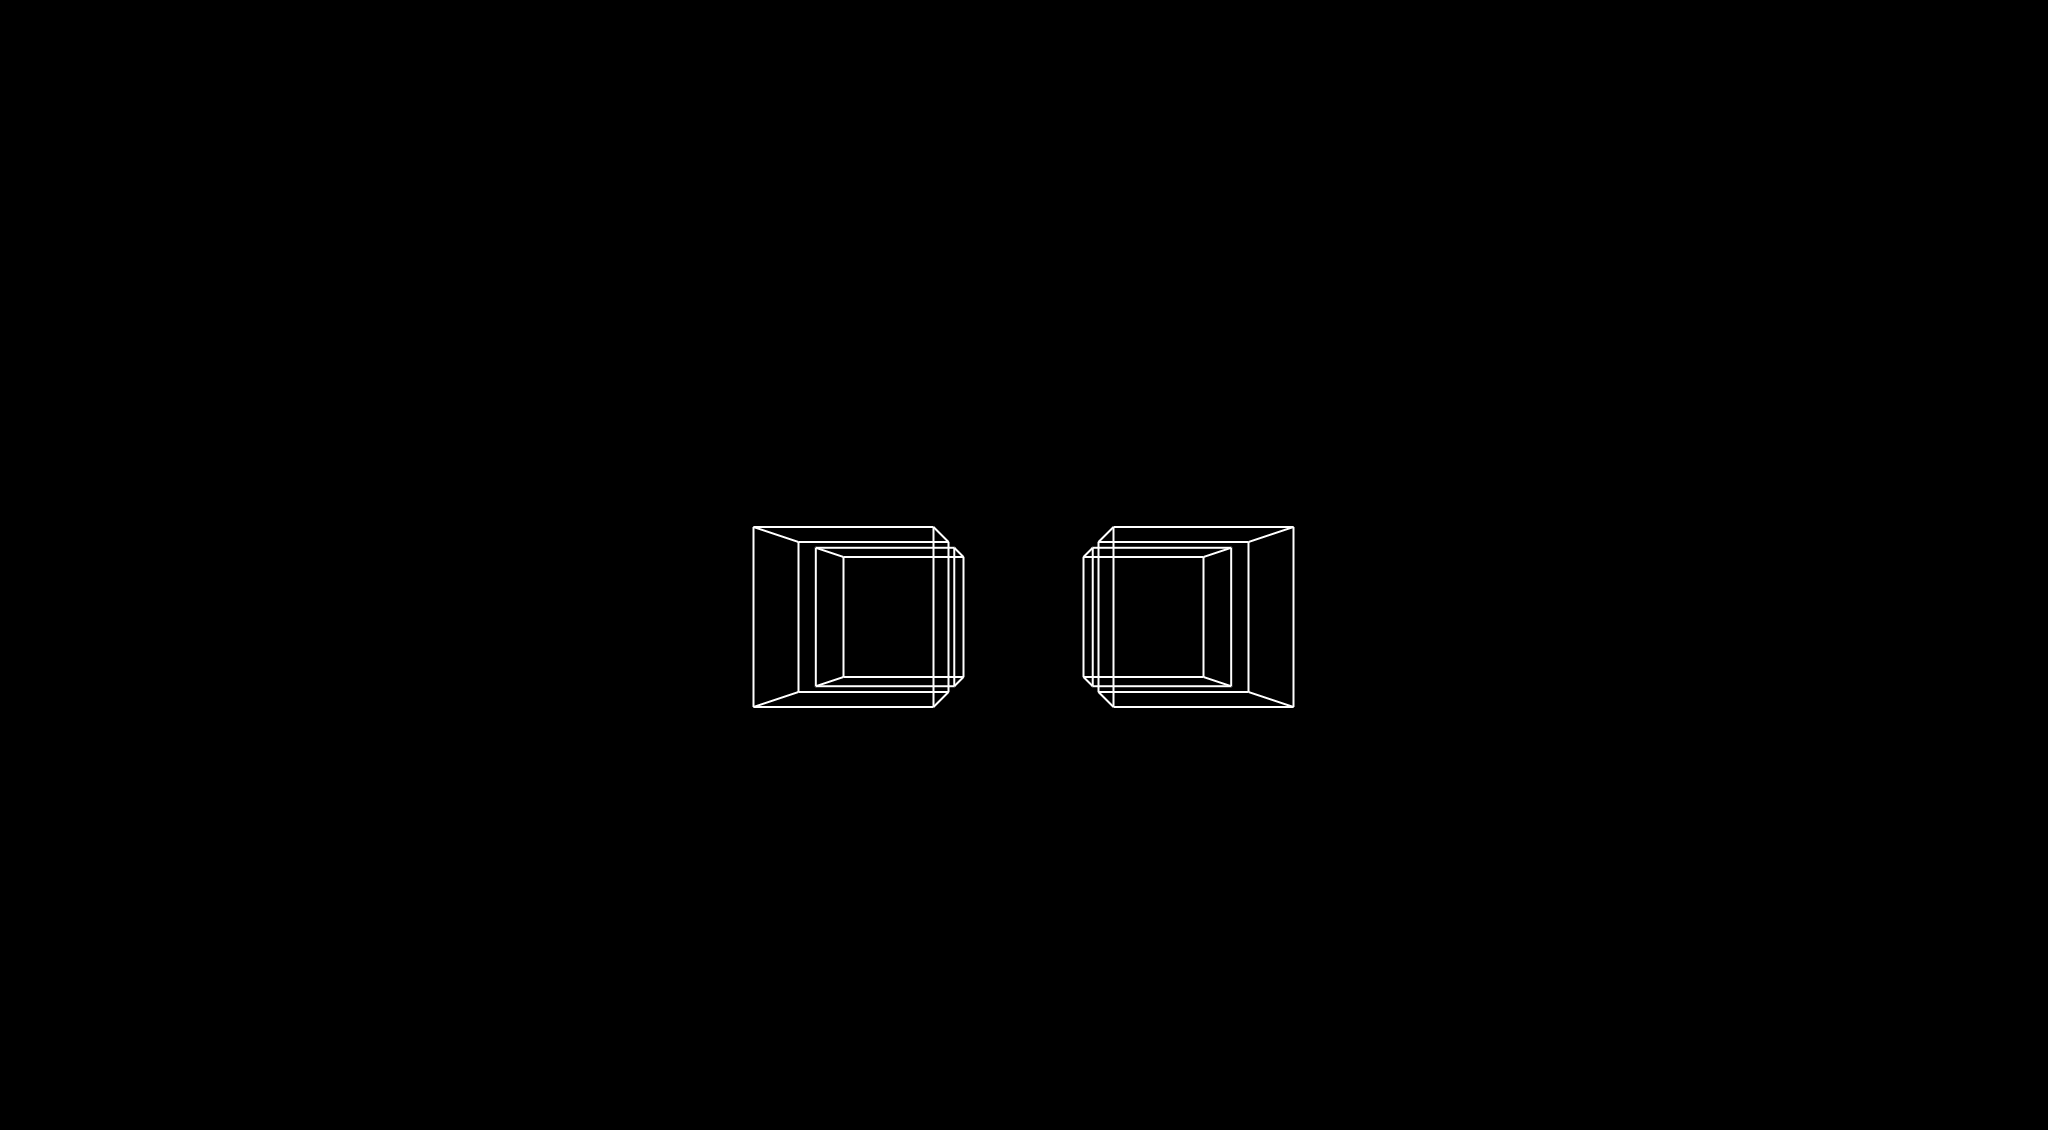
\includegraphics[width=\textwidth]{original}
        \caption{Początkowe wyświetlenie obiektów}
        \centering
    \end{figure}

\newpage

    \subsection{Translacja}
    
        Macierz translacji:

        \begin{equation}
            M_t=
            \begin{bmatrix}
                1 & 0 & 0 & x_t \\
                0 & 1 & 0 & y_t \\
                0 & 0 & 1 & z_t \\
                0 & 0 &0 & 1
            \end{bmatrix}
        \end{equation}

        Gdzie \(x_t, y_t, z_t\) -- kolejne współrzędne translacji obiektu.

        \begin{figure}[h]
            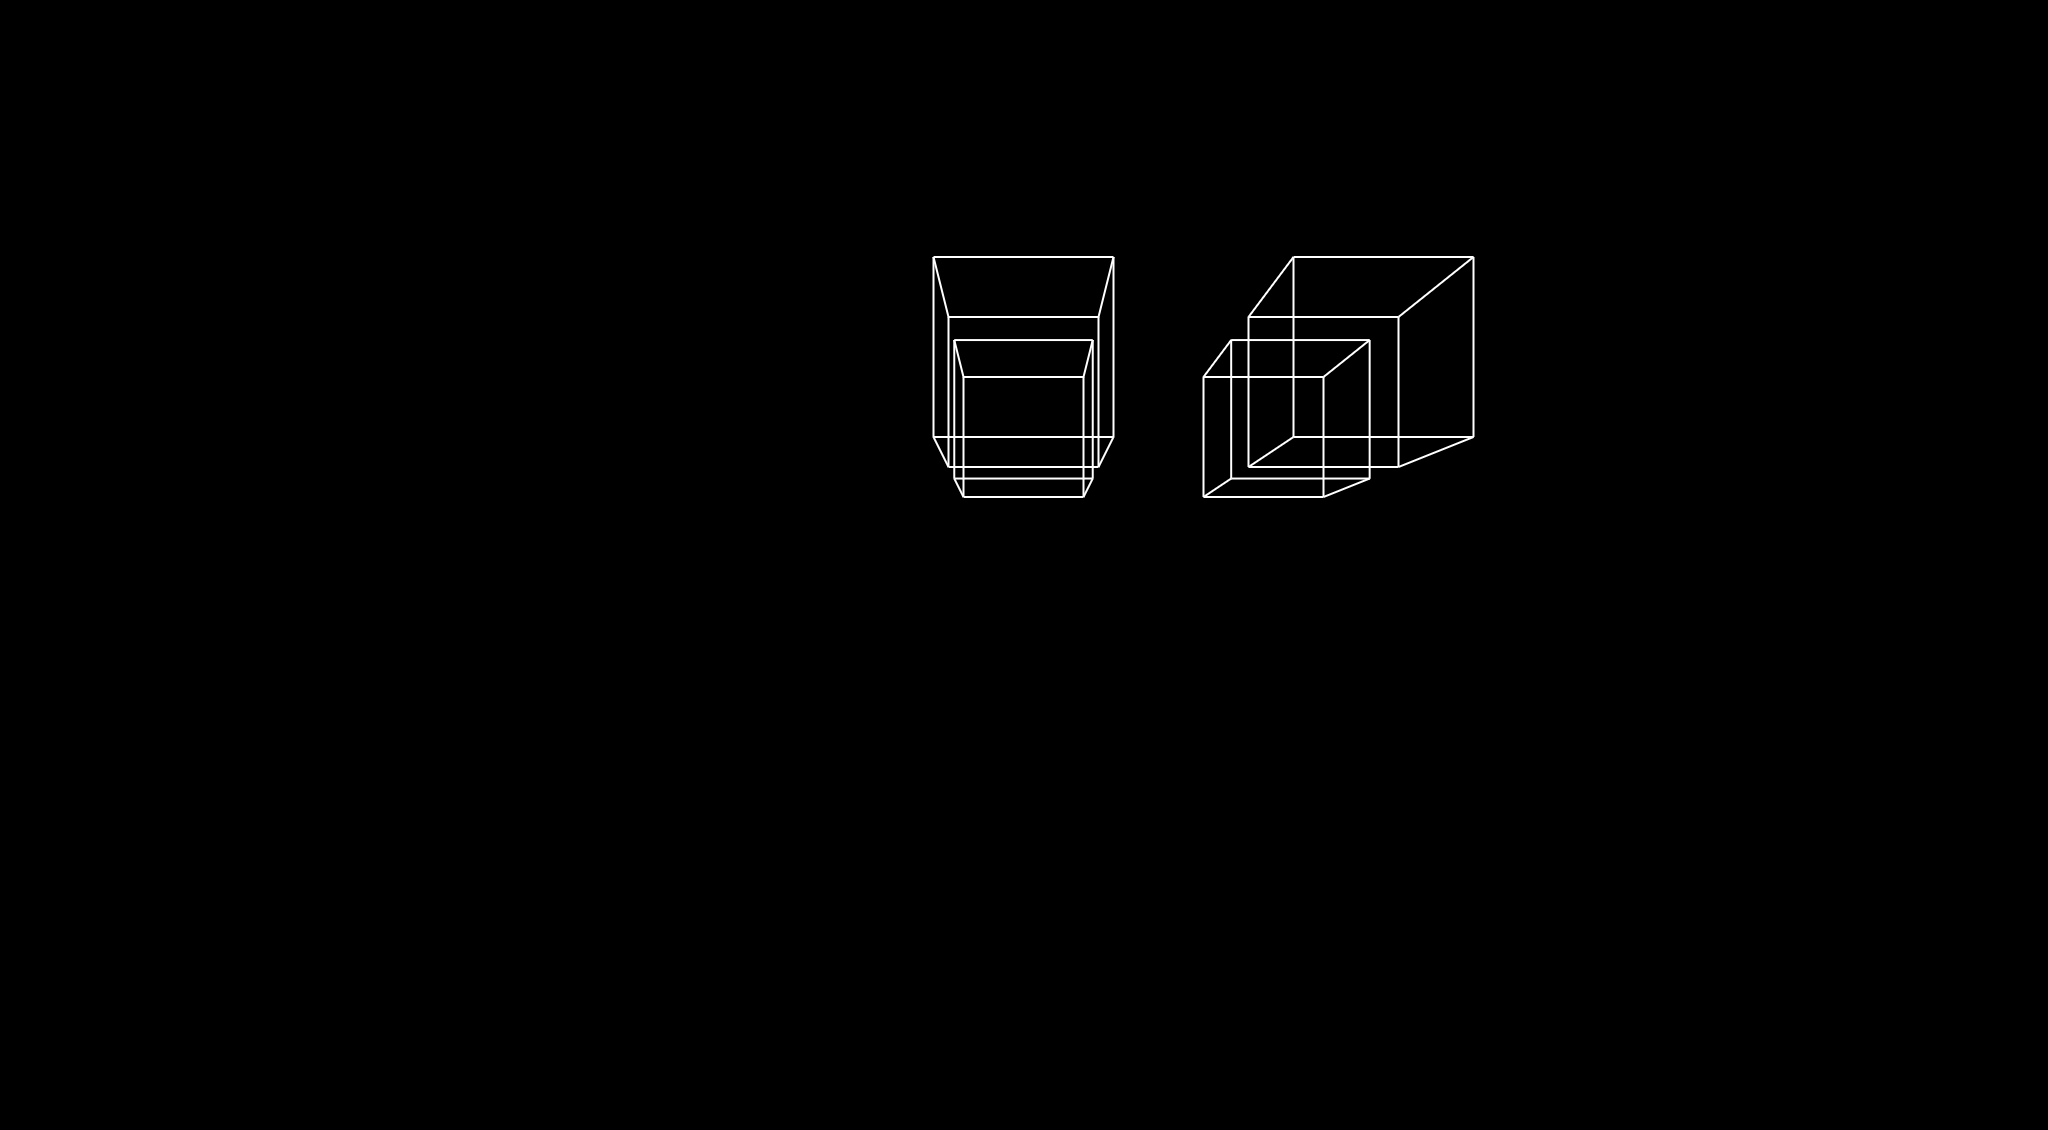
\includegraphics[width=\textwidth]{translation}
            \caption{Obiekty poddane translacji \(x_t, y_t\)}
            \centering
        \end{figure}

    \subsection{Rotacja}

        \begin{figure}
            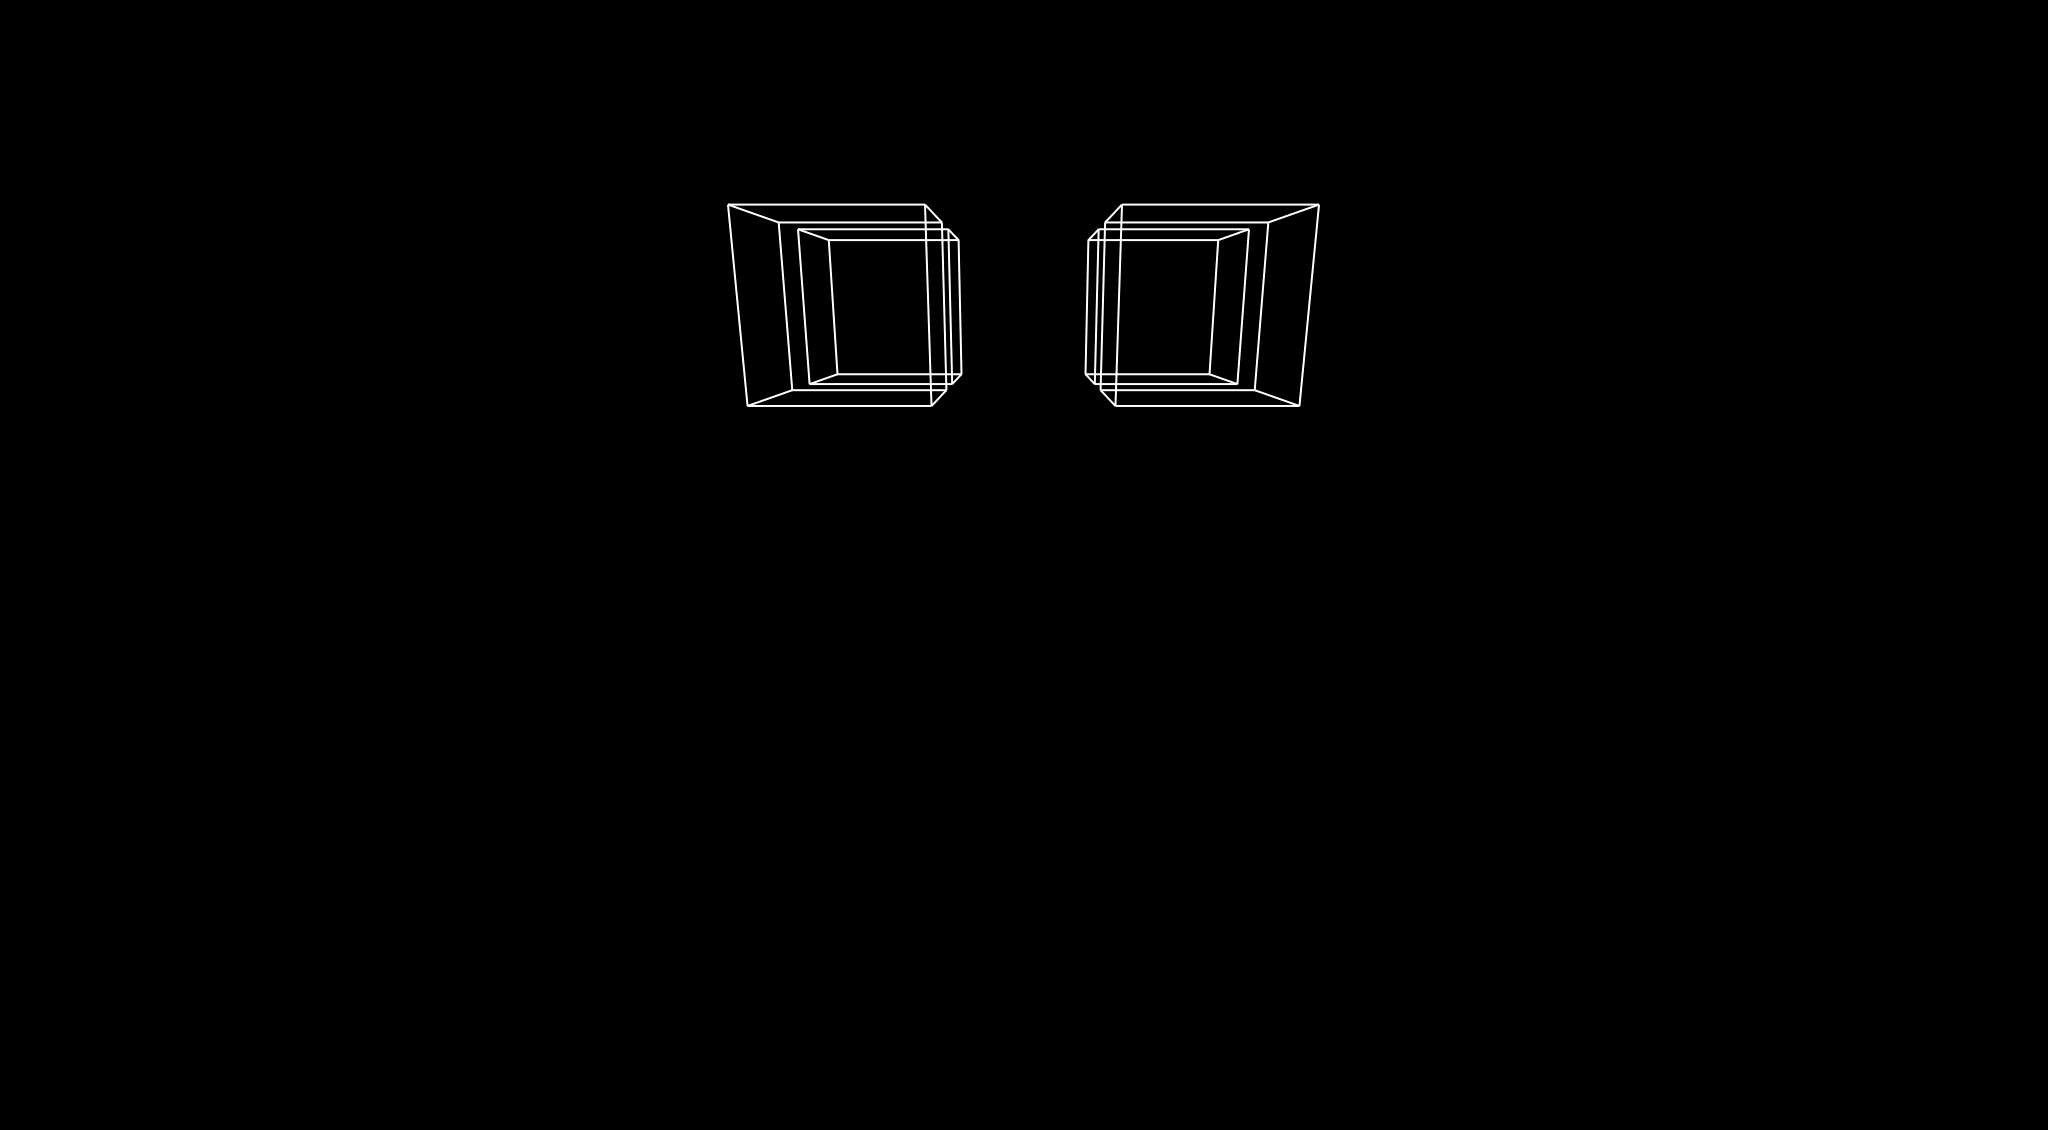
\includegraphics[width=\textwidth]{rotate_x}
            \caption{Obiekty poddane rotacji względem osi \(x\)}
            \centering
        \end{figure}

        \begin{figure}
            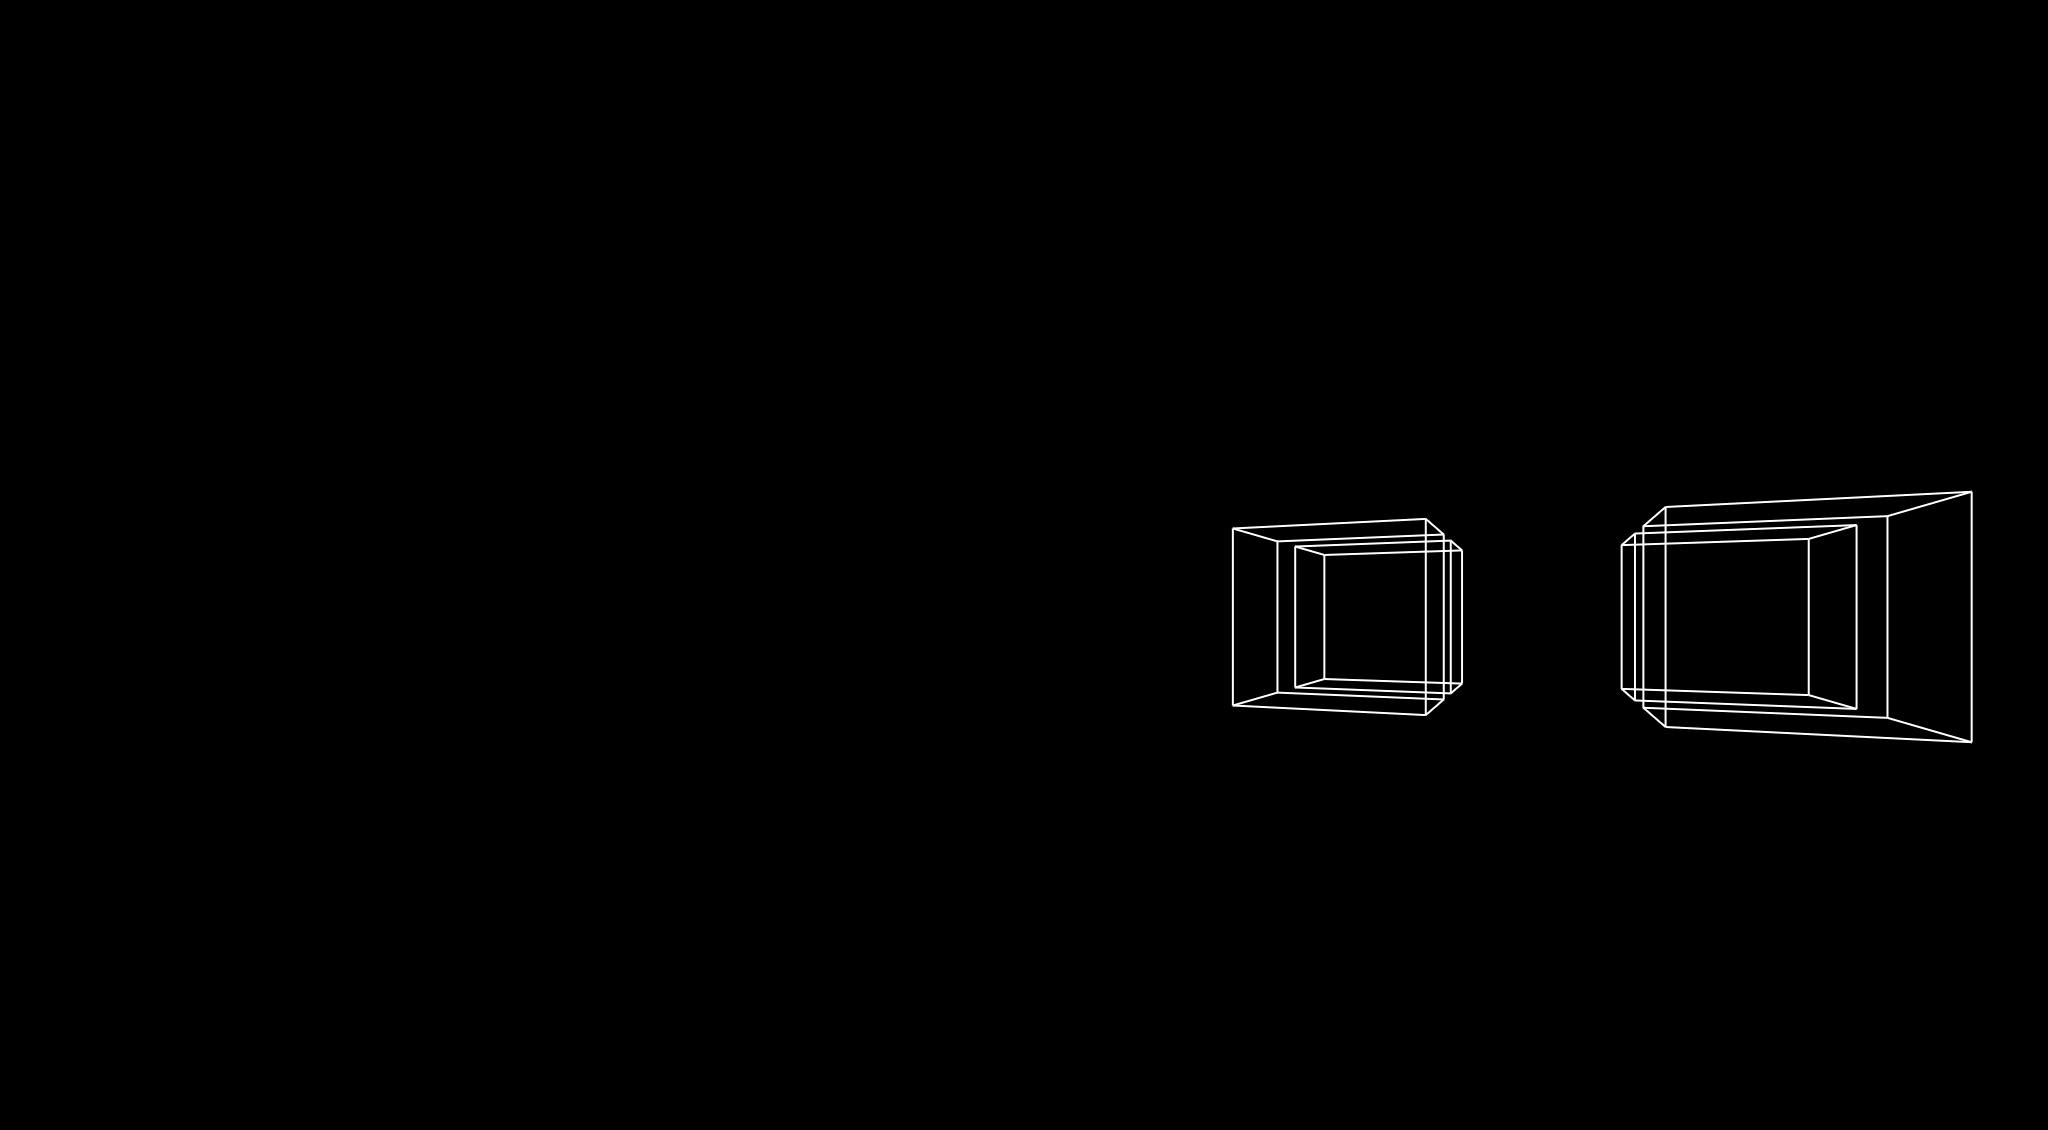
\includegraphics[width=\textwidth]{rotate_y}
            \caption{Obiekty poddane rotacji względem osi \(y\)}
            \centering
        \end{figure}

        \begin{figure}
            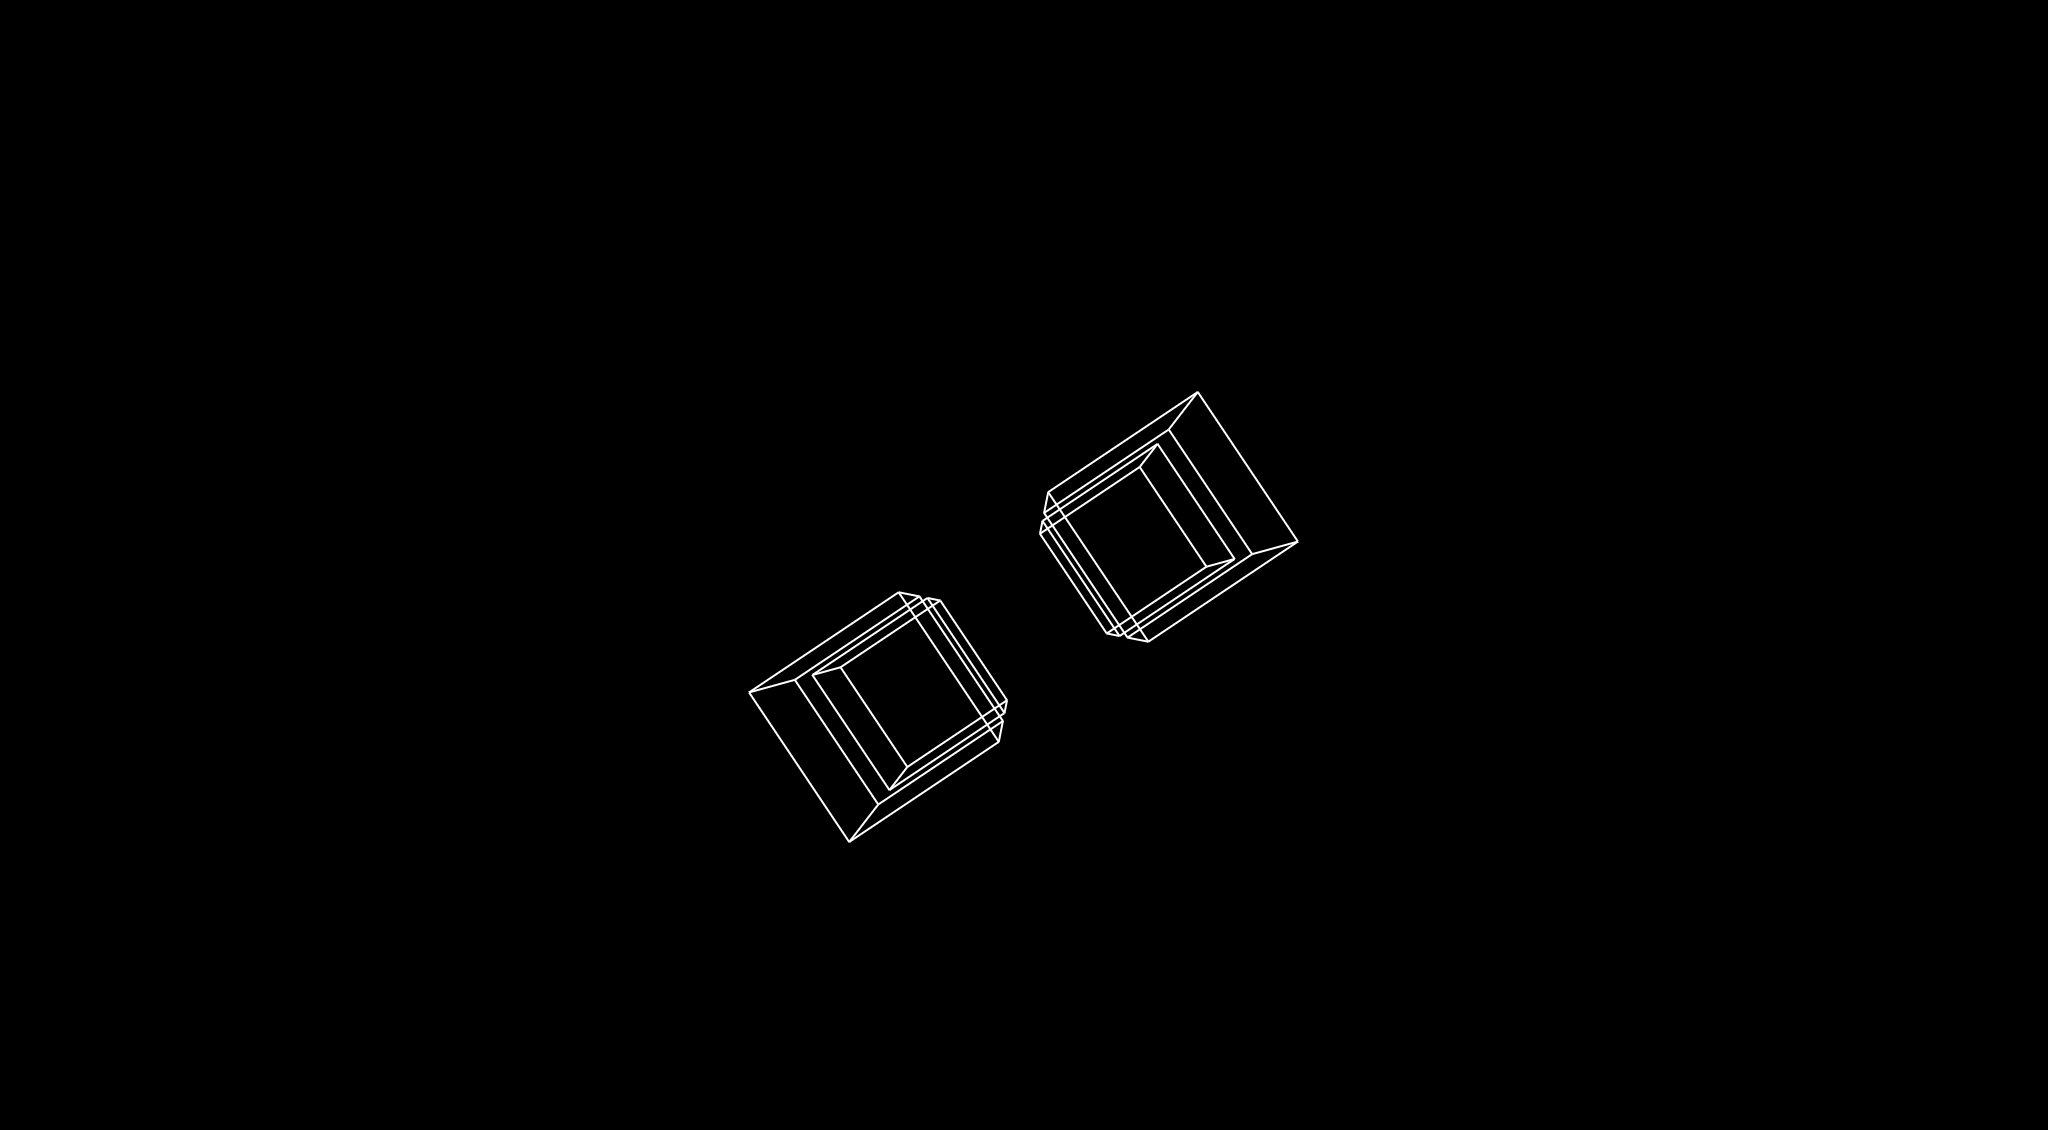
\includegraphics[width=\textwidth]{rotate_z}
            \caption{Obiekty poddane rotacji względem osi \(z\)}
            \centering
        \end{figure}

        Macierze rotacji:

        \begin{equation}
            M_{rx}=
            \begin{bmatrix}
                1 & 0 & 0 & 0 \\
                0 & cos(\alpha) & sin(\alpha) & 0 \\
                0 & -sin(\alpha) & cos(\alpha) & 0 \\
                0 & 0 & 0 & 1
            \end{bmatrix}
        \end{equation}

        \begin{equation}
            M_{ry}=
            \begin{bmatrix}
                cos(\alpha) & 0 & -sin(\alpha) & 0 \\
                0 & 1 & 0 & 0 \\
                sin(\alpha) & 0 & cos(\alpha) & 0 \\
                0 & 0 & 0 & 1
            \end{bmatrix}
        \end{equation}

        \begin{equation}
            M_{rz}=
            \begin{bmatrix}
                cos(\alpha) & sin(\alpha) & 0 & 0 \\
                -sin(\alpha) & cos(\alpha) & 0 & 0 \\
                0 & 0 & 1 & 0 \\
                0 & 0 & 0 & 1
            \end{bmatrix}
        \end{equation}

        Gdzie \(x, y, z\) -- osie rotacji.

    \subsection{Zoom}

        \begin{figure}
            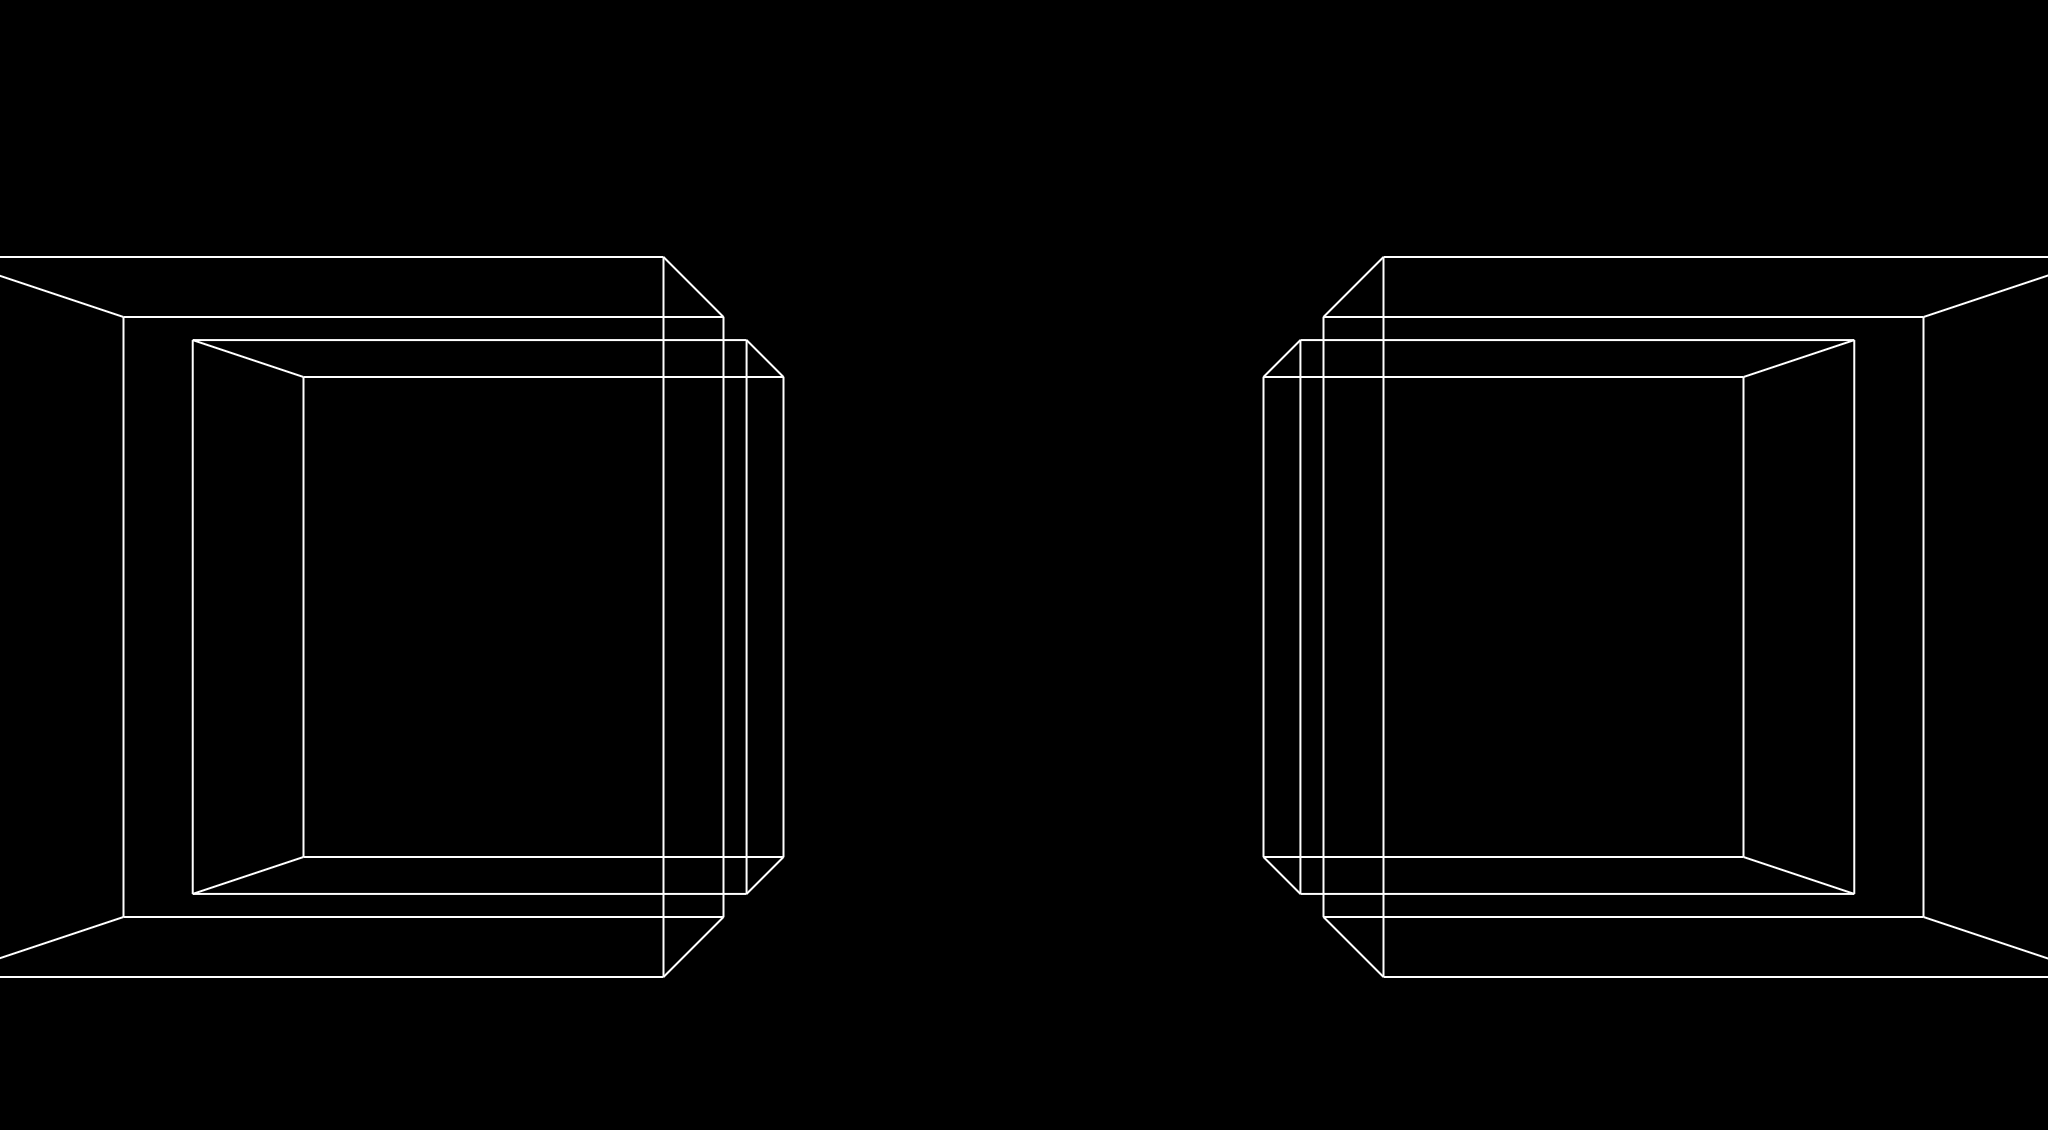
\includegraphics[width=\textwidth]{zoom_in}
            \caption{Obiekty poddane operacji zoom (\(z > 1\))}
            \centering
        \end{figure}

        \begin{figure}
            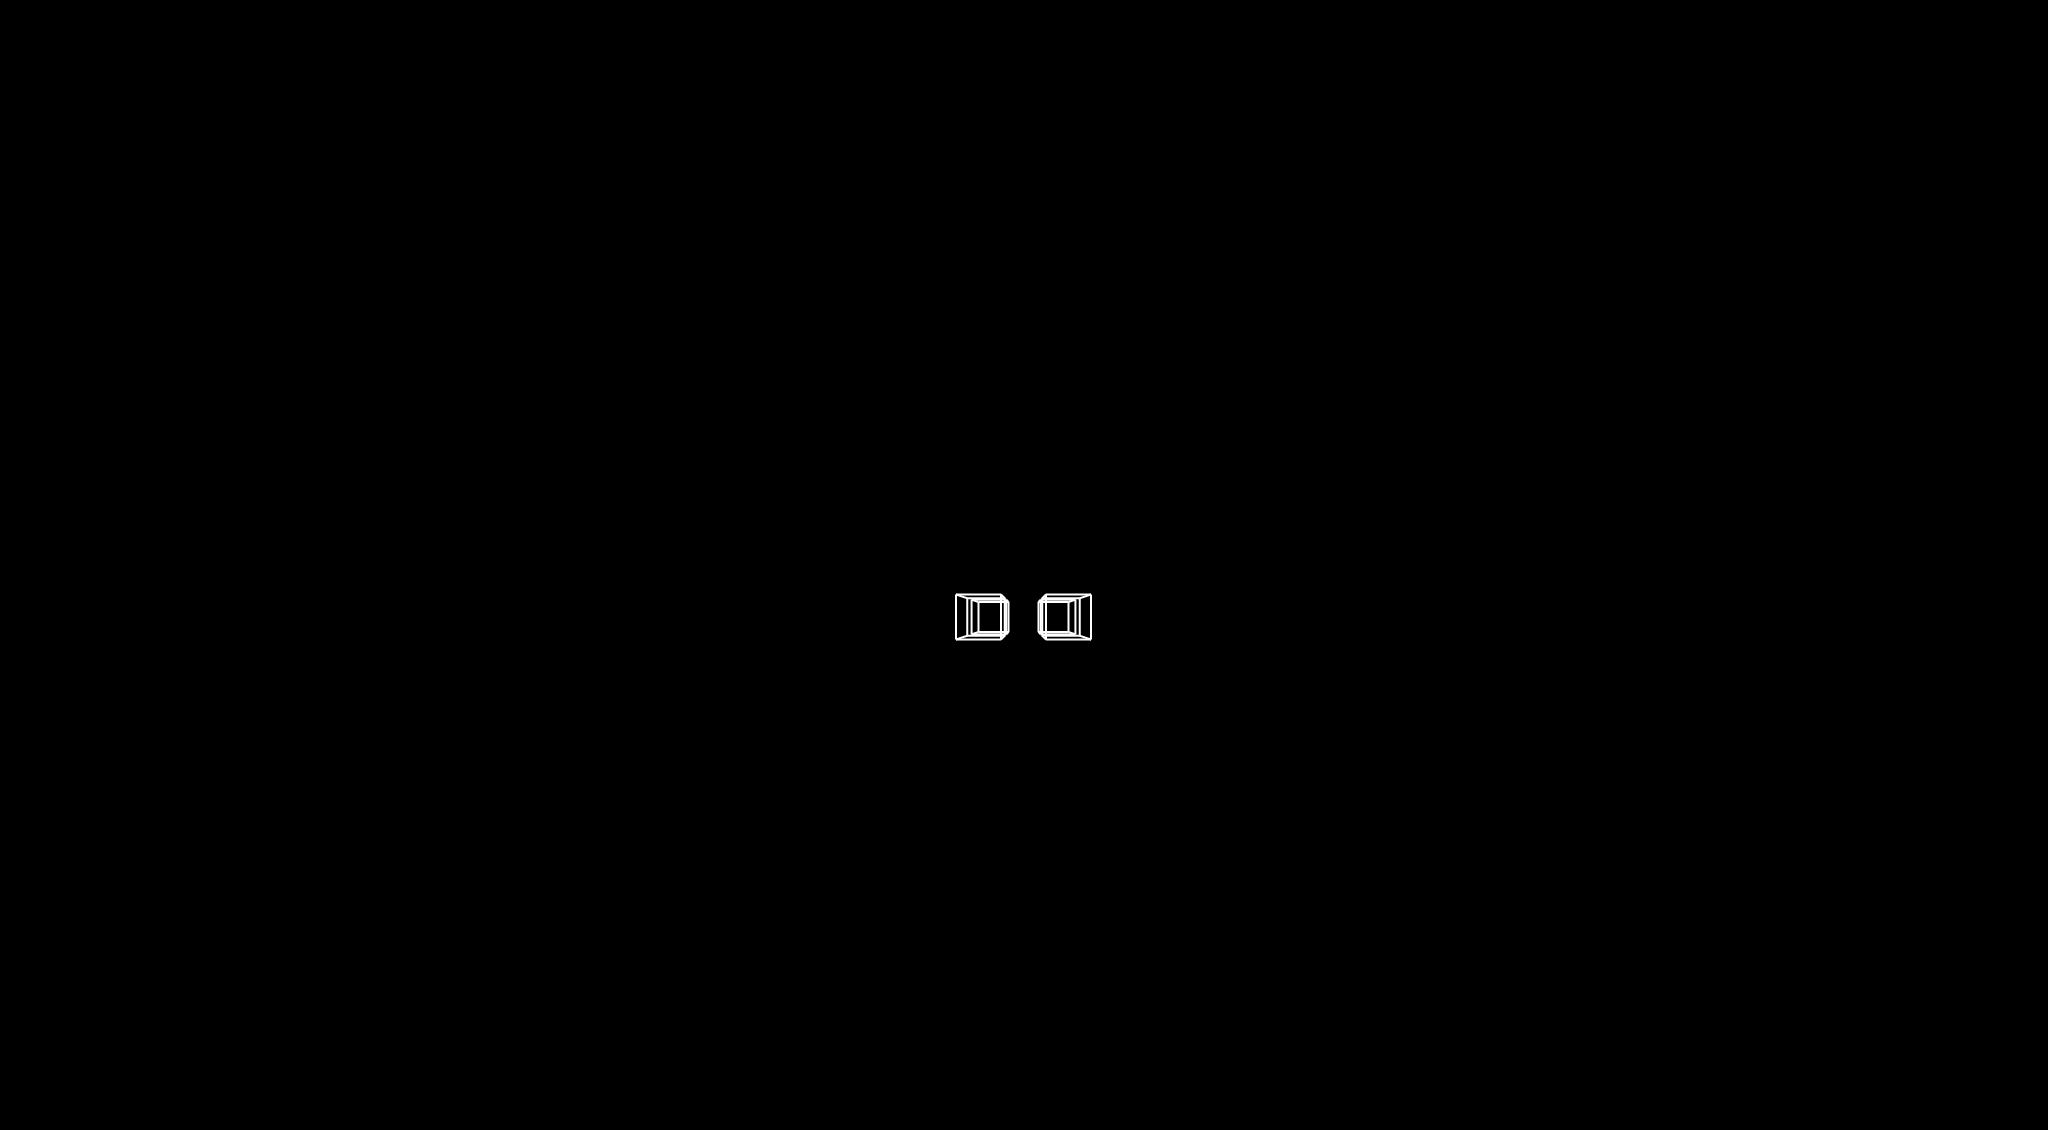
\includegraphics[width=\textwidth]{zoom_out}
            \caption{Obiekty poddane operacji zoom (\(z > 0\) i \(z < 1\))}
            \centering
        \end{figure}

        Macierz operacji zoom:

        \begin{equation}
            M_t=
            \begin{bmatrix}
                z & 0 & 0 & 0 \\
                0 & z & 0 & 0 \\
                0 & 0 & 1 & 0 \\
                0 & 0 &0 & 1
            \end{bmatrix}
        \end{equation}

        Gdzie \(z\) -- stopień powiększenia.

\newpage

\section{Odwzorowanie punktu 3D na powierzchni 2D}

    Odwzorowanie następuje poprzez przemnożenie punktów z kolejnymi macierzami:

    \begin{enumerate}

        \item Przejście z układu współrzędnych kamery do \textit{canonical view volume} wraz 
        z transformacją perspektywistyczną (\(orth\_to\_canonical * perspective\_matrix\)).

        \begin{equation}
            M_{per}=
            \begin{bmatrix}
                \frac{2n}{r-l} & 0 & \frac{l+r}{l-r} & 0 \\
                0 & \frac{2n}{t-b} & \frac{b+t}{b-t} & 0 \\
                0 & 0 & \frac{f+n}{n-f} & \frac{2fn}{f-n} \\
                0 & 0 & 1 & 0
            \end{bmatrix}
        \end{equation}

        Gdzie \(l, r, t, b, n, f\) -- wymiary \textit{orthographic view volume} (left, right,
        top, bottom, near, far).

        \item \textit{Viewport transformation} -- przejście z \textit{canonical view volume}
        do wymiarów canvasa (bez zmiany \(z\)).

        \begin{equation}
            M_{vp}=
            \begin{bmatrix}
                \frac{n_x}{2} & 0 & 0 & \frac{n_x-1}{2} \\
                0 & \frac{n_y}{2} & 0 & \frac{n_y-1}{2} \\
                0 & 0 & 1 & 0 \\
                0 & 0 & 0 & 1
            \end{bmatrix}
        \end{equation}

        Gdzie \(n_x, n_y\) -- rozmiary canvasa.

    \end{enumerate}

\section{Wnioski}

    W wykonaniu ćwiczenia niepotrzebnie wykorzystano transformację z układu współrzędnych
    kamery do \textit{canonical view volume} -- można było zastosować prostsze macierze. 
    Będzie to przydatne w wykonaniu drugiej części projektu do usuwania powierzchni zakrytych.
 
\end{document}
